\section{Enmascaramiento Cuantitativo} \label{sec:QuantMask_mask}
En esta sección, extendemos el juego de simulación de enmascaramiento fuerte (resp. débil) introducido anteriormente con objetivos cuantitativos para así definir la noción de distancia de tolerancia a fallas enmascarante.
% In practice, fault-tolerance appears with a quantitative flavor, that is, fault-tolerant systems have %degrees of tolerance. This is particularly true when techniques like redundancy and voting are used.  %take this into account. 
Es importante remarcar que en este capítulo utilizamos el atributo  ``cuantitativo'' en un sentido no probabilista.
\begin{definition}  
  %Let $A=\langle S, \Sigma, E, s_0\rangle$ and $A'=\langle S', \Sigma_{\Faults}, E', s'_0 \rangle$.  T
  Para los sistemas de transición $A$ y $A'$, el \emph{grafo de juego de enmascaramiento cuantitativo fuerte} 
  $\QMStrGame = \langle V^G, V_\Refuter, V_\Verifier, E^G,  \InitVertex^G,  \reward^G \rangle$ se define de la siguiente manera:
 
\begin{itemize}
\item
  $\mathcal{G}_{A, A'}=\langle V^G, V_\Refuter, V_\Verifier, E^G, \InitVertex^G \rangle$ se define como en Definición~\ref{def:strong_masking_game_graph},
\item
  $ \reward^G(v) = (\chi_{\Faults}(\pr{1}{v}), \chi_{\ErrorSt}(v))$

\end{itemize}
%
donde $\chi_{\Faults}$ es la función característica sobre el conjunto $\Faults$, devolviendo $1$ si $\sigma \in \Faults$ y $0$ de otro modo, y $\chi_{\ErrorSt}$ es la función característica sobre el conjunto unitario $\{\ErrorSt\}$.
\end{definition}
Observemos que la función de recompensa retorna un par de números en lugar de un solo número. Es directo codificar al par como un único numero pero no lo hacemos por claridad. Remarcamos que el
\emph{grafo de juego de enmascaramiento cuantitativo débil} $\QMWeakGame$
se define de la misma forma que el grafo de juego definido arriba pero utilizando el grafo de juego de enmascaramiento débil $\mathcal{G}^W_{A, A'}$ en lugar de 
$\mathcal{G}_{A, A'}$


Dado un grafo de juego de enmascaramiento cuantitativo fuerte con la función de recompensa $\reward^G$ y la jugada 
$\rho = \rho_0 \rho_1 \rho_2, \ldots$, para todo $i \geq 0$, sea 
%$v_i = v^G(\rho_i \xrightarrow{\sigma_i} \rho_{i+1})$.
$r_i = \reward^G(\rho_i)$.
Definimos la \emph{función de payoff de enmascaramiento} de la siguiente manera: 
\[%\displaystyle
\FMask(\rho) = \lim_{n \rightarrow \infty}  \frac{\pr{1}{r_n}}{1+ \sum^{n}_{i=0} \pr{0}{r_i}},
%\FMask(\rho) = \liminf_{n \rightarrow \infty}  \frac{\pr{1}{v_n}}{1+ \sum^{n}_{i=0} \pr{0}{v_i}},
\]
la cual es proporcional a la inversa de la cantidad de movimientos de enmascaramiento realizados por el Verificador. Para entender esto, notemos que el numerador de $\frac{\pr{1}{r_n}}{1+ \sum^{n}_{i=0} \pr{0}{r_i}}$ será $1$
cuando alcancemos el estado de error, es decir, en aquellos caminos que no alcancen el estado de error esta fórmula devuelve $0$. Además, si el estado de error es alcanzado,  el denominador contará el número de transiciones de falla tomadas hasta el estado de error. Todas, a excepción de la última fueron enmascaradas exitosamente. Sin embargo, la última falla tratara de ser enmascarada por el Verificador, pero eventualmente llevará al estado de error.
Es decir, los vértices con valor $(1,\_)$ son aquellos correspondientes a fallas. Los demás se corresponden con $(0,\_)$.
Observemos también que si $\ErrorSt$ es alcanzado en $v_n$ sin la ocurrencia de ninguna falla, la parte nominal de la implementación no se corresponde con la especificación nominal, en cuyo caso $\frac{\pr{1}{r_n}}{1+ \sum^{n}_{i=0} \pr{0}{r_i}}=1$.
Entonces, el Refutador quiere maximizar el valor de cualquier jugada, es decir, tratará de alcanzar al estado $\ErrorSt$ bajo la menor cantidad de fallas, y por lo tanto enmascaramientos, posibles. 
Por el contrario, el Verificador quiere evitar $\ErrorSt$ y entonces tratará de enmascarar fallas de tal forma que se aleje del estado de error. 

Formalmente, el valor del juego de enmascaramiento cuantitativo fuerte para el Refutador se define como $\val_\Refuter(\QMStrGame) = \Sup_{\pi_\Refuter \in \Pi_\Refuter} \; \Inf_{\pi_\Verifier \in \Pi_\Verifier} \FMask(\out(\pi_\Refuter, \pi_\Verifier))$. De forma análoga, el valor del juego para el Verificador se define como $\val_\Verifier(\QMStrGame) = \Inf_{\pi_\Verifier \in \Pi_\Verifier} \; \Sup_{\pi_\Refuter \in \Pi_\Refuter} \FMask(\out(\pi_\Refuter, 
\pi_\Verifier))$. Entonces, definimos el valor del juego de enmascaramiento cuantitativo fuerte, denotado por $\val(\QMStrGame)$, como el valor del juego del Refutador o del Verificador, es decir, $\val(\QMStrGame) = \val_\Refuter(\QMStrGame) = \val_\Verifier(\QMStrGame)$. Esto es posible debido a que los juegos de enmascaramiento cuantitativos fuertes están determinados como lo probaremos mas adelante en el Teorema~\ref{thm:mask_game_det}. \\

\begin{definition} \label{def:mask_dist}
 Sean $A$ y $A'$ unos sistemas de transición. 
La \emph{distancia de enmascaramiento fuerte} entre $A$ y $A'$, denotada por $\DeltaMask(A, A')$ se define de la siguiente manera:
$\DeltaMask(A, A') = \val(\QMStrGame).$
\end{definition}

Es necesario remarcar que la \emph{distancia de enmascaramiento débil} $\DeltaMask^W$ se define de la misma forma para el grafo de juego de enmascaramiento cuantitativo débil $\QMWeakGame$.  A grandes rasgos, estamos interesados en medir la cantidad de fallas que pueden ser enmascaradas. El valor del juego está esencialmente determinado por las transiciones de falla en el grafo de juego y por cómo los jugadores pueden encontrar una estrategia que lleve a (o evite) el estado $\ErrorSt$, independientemente de la existencia de acciones silenciosas.

A continuación, estableceremos algunas propiedades básicas de este tipo de juegos. 
Como ya anticipamos, los juegos de enmascaramiento cuantitativos fuertes están determinados.

\begin{theorem} \label{thm:mask_game_det}
  Para cualquier grafo de juego de enmascaramiento cuantitativo fuerte $\QMStrGame$ con función de \textit{payoff} $\FMask$:
%  \vspace{-0.3cm}
  \[\textstyle
  \Inf_{\pi_\Verifier \in \Pi_\Verifier} \; \Sup_{\pi_\Refuter \in \Pi_\Refuter} \FMask(\out(\pi_\Refuter, \pi_\Verifier)) = \Sup_{\pi_\Refuter \in \Pi_\Refuter} \;  \Inf_{\pi_\Verifier \in \Pi_\Verifier} \FMask(\out(\pi_\Refuter, \pi_\Verifier))\]
\end{theorem}
\begin{proof} Para demostrar que la función de \textit{payoff} de enmascaramiento $\FMask$ está determinada tenemos que probar que está acotada y que es Borel-medible (teorema de Martin \cite{Martin98}). Primero, $\FMask$ está acotada por definición. Segundo, para ver que $\FMask$ es Borel-medible notemos que $\FMask(\Omega) \subseteq [0,1]$, y entonces es suficiente para probar que, para cada racional $x$, $\FMask^{-1}((-\infty, x])$ es Borel en la topología de Cantor de ejecuciones infinitas. 
Consideremos $\FMask^{-1}([-\infty,x])$ para un $x$ arbitrario, esto es lo mismo que $\FMask^{-1}([0, \frac{1}{a}])$ para un $a$ dado. Pero, $\FMask^{-1}([0, \frac{1}{a}]) = \bigcup_{b \geq a} A_b$ donde
$A_b = \bigcup_{i >0} A^i_b$ para $A^i_b = \{ \rho_0 \rho_1 \dots \mid \rho_i = \ErrorSt \wedge \sum^{i-1}_{j=0} \chi_{\Faults}(\pr{1}{\rho_j}) =b\}$. Notemos que 
$A^i_b = \{ C_{\rho_0 \dots \rho_i} \mid \sum^{i-1}_{j=0} \chi_{\Faults}(\pr{1}{\rho_j}) =b\}$ donde $C_{\rho_0 \dots \rho_i}$ es el cono correspondiente al segmento inicial 
$\rho_0 \dots \rho_i$ el cuál es Borel-medible, y por lo tanto $A^i_b$, $A_b$ y $\FMask^{-1}((-\infty, x])$ son Borel-medibles.
\qedhere
%is the set of all sequences $x_0 x_1 x_2 \dots$
%such that we have $b$ or more ones, and this is the union $\bigcup A_i$ being $A_i = \{\sigma \mid \mbox{ number of ones of } \sigma[0,i] = b\}$, which are Borel sets, thus $A$ is a Borel set.
\end{proof} \\


\subsection{Cómputo de la Distancia de Enmascaramiento}

En esta subsección presentamos los algoritmos para computar la distancia de enmascaramiento para un juego de enmascaramiento cuantitativo fuerte (resp. débil). Mostramos que, en el caso de sistemas deterministas, computar la distancia de enmascaramiento puede ser logrado utilizando un algoritmo de camino más corto. A diferencia de los sistemas no deterministas, en cuyo caso el cómputo puede ser realizado por un algoritmo de punto fijo.

Comenzamos presentando el próximo teorema que establece como se calcula el valor de un juego de enmascaramiento cuantitativo fuerte dado.
%

\begin{theorem} \label{thm:quant_game}
  Sea $\QMStrGame$ un grafo de juego de enmascaramiento cuantitativo fuerte.
  \sloppy Entonces, $\val(\QMStrGame) = \frac{1}{\pr{0}{\delta(\InitVertex^G)}}$, con
  $\delta(\InitVertex^G) = \min \{ (i,j) \mid  \InitVertex^G \in \setsUs \}$, siempre que
  $\InitVertex^G \in U$, y $\val(\QMStrGame)=0$ de otro modo, donde los conjuntos
   $\setsUs$ y $U$ están definidos en Definición~\ref{def:U}.

\end{theorem}
% PRUEBA PASADA AL APENDICE
\iffalse
\begin{proof} La prueba es por casos:
	
	Si $\InitVertex^G \notin U$, entonces definimos la siguiente estrategia para el Verificador. Si $v \in V_\Verifier \setminus U$, entonces $\pi^*_\Verifier(v)=v'$ 
	para algún $v' \in V_\Refuter \setminus U$, y si $v \notin  V_\Verifier \setminus U$, entonces $\pi^*_\Verifier(v) = v'$ para un $v'$ arbitrario. 
	Probamos por inducción que para cualquier jugada que se conforme a $\pi^*_\Verifier$: $\rho =\rho_0 \rho_1 \dots$ tenemos $\forall i \geq 0: \rho_i \notin V \setminus U$. El caso base es directo. 
Para el caso inductivo, asumamos que $\rho_i \notin V \setminus U$. En caso que $\rho_i \in V_\Verifier$, la propiedad se deduce por definición de
$\pi^*_\Verifier$. Si $\rho_i \in V_\Refuter$, como $\rho_i \in V^G \setminus U$, entonces $\post(\rho_i) \subseteq V^G \setminus U$ (por Definición~\ref{def:U}). 
Por lo tanto, $\rho_{i+1} \in V^G \setminus U$. 
	 Además, también tenemos $\rho_i \neq \ErrorSt$ ya que $\{ \ErrorSt \} \subseteq U$. También note que cualquier jugada que evite el estado $\ErrorSt$ tiene valor $0$: por definición de $\QMStrGame$, cada transición ejecutada por el Refutador debe ser sucedida por una transición seleccionada por el Verificador. Estas transiciones (las elegidas por el Verificador) tienen costo $(1,0)$ ya que el destino de cualquiera de estas transiciones es diferente de $\ErrorSt$. Como tenemos una cantidad infinita de estos movimientos del Verificador, cuando el estado $\ErrorSt$ no es alcanzado, la valuación de estas jugadas es $\lim_{n\rightarrow \infty} \frac{0}{1+ \sum^n_{i=0} \pr{0}{r_i}} = 0$ (recordemos que $r_i = \reward^G(\rho_i)$). 
En resumen, $\sup_{\pi_\Refuter \in \Pi_\Refuter} \FMask(\out(\pi_\Refuter, \pi^*_\Verifier)) = 0$, y como $\FMask$ es positiva
tenemos $\val(\QMStrGame) = \inf_{\pi_\Verifier \in \Pi_\Verifier} \sup_{\pi_\Refuter \in \Pi_\Refuter} \FMask(\out(\pi_\Refuter, \pi_\Verifier)) = 0$.

	Si $\InitVertex^G \in U$, tenemos que $\delta(\InitVertex^G) < (\infty, \infty)$, entonces definimos la siguiente estrategia para el Refutador. 
	Si $v \in U$, entonces $\pi^*_\Refuter(v)= v'$, donde $\delta(v') < \delta(v)$, sino $\pi^*_\Refuter(v)=v'$, para un $v'$ arbitrario. 
	La estrategia $\pi^*_R$ esta bien definida ya que si $v \in \setsUs$, entonces existe un $v' \in \post(v)$ tal que $v \in U^{j-1}_i$ (por Definición~\ref{def:U}). Además, $\delta(v') = (\pr{0}{\delta(v)}, \pr{1}{\delta(v)} - 1)$.  
	Ahora bien, probaremos que para cada estrategia $\pi_\Verifier \in \Pi_\Verifier$ tal que $\out(\pi^*_\Refuter, \pi_\Verifier) = \rho = \rho_0 \rho_1 \dots$ y $\rho_0 \in U$, tenemos:
\begin{equation}\label{eq:inf-bound}
	\FMask(\out(\pi^*_\Refuter, \pi_\Verifier)) \geq \frac{1}{ \pr{0}{\delta(\rho_0)}}
\end{equation} 
		Para demostrar esto, note que, si $\delta(\rho_0)= (i,j)$, entonces $\rho_j =\ErrorSt$ 
		ya que $\pr{1}{\delta(\rho_k)} = \pr{1}{\delta(\rho_{k+1})}+1$ para todo $k$. 
Esto significa que, en $j$ pasos tenemos $\delta(\rho_{j}) = (1,1)$ y entonces $\rho_{j} = \ErrorSt$.
	Esto implica que $\FMask(\rho) =  \lim_{n \rightarrow \infty}  \frac{\pr{1}{r_n}}{1+ \sum^{n}_{i=0} \pr{0}{r_i}} >0$, y también
$ \sum^{\pr{1}{\delta(\rho_0)} + k}_{i=0} \pr{0}{r_i} =  \sum^{\pr{1}{\delta(\rho_0)}}_{i=0} \pr{0}{r_i}$.
	 Es decir, probando que:
\begin{equation}\label{eq:bottom-sum}
 1+ \sum^{\pr{1}{\delta(\rho_0)}}_{i=0} \pr{0}{r_i} \geq \pr{0}{\delta(\rho_0)}
\end{equation} 
tenemos $\FMask(\rho) \geq \frac{1}{ \pr{0}{\delta(\rho_0)}}$. La prueba es por inducción sobre $\delta(\rho_0)$, el caso base es directo.
 Para el caso inductivo, si $\rho_0 \in V_\Refuter$, entonces
\begin{align*}
 	1 + \sum^{\pr{1}{\delta(\rho_0)}}_{i=0} \pr{0}{r_i} & =  1 + \pr{0}{r_0} + \sum^{\pr{1}{\delta(\rho_0)}}_{i=1} \pr{0}{r_i} & \\
					   %  & =   1+\sum^{\pr{1}{\delta(\rho_0)}}_{i=1} \pr{0}{r_i} & \\
					    % & =   1+\sum^{\pr{1}{\delta(\rho_1)}+1}_{i=1} \pr{0}{r_i} & \\
					     & =   1+ \sum^{\pr{1}{\delta(\rho_1)}}_{i=0} \pr{0}{r_{i+1}} &  \text{($\rho_0 \in V_\Refuter$)}\\
					     & \geq \pr{0}{\delta(\rho_1)} & \text{(I.H.)} \\
					     & = \pr{0}{\delta(\rho_0)} & \text{($\rho_0 \in V_\Refuter$)}
\end{align*}
 Si $\rho_0 \in V_\Verifier$ y $\pr{1}{\rho_0} \notin \Faults$, entonces la prueba es como arriba. Si $\pr{1}{\rho_0} \in \Faults$, entonces:
\begin{align*}
 	1+\sum^{\pr{1}{\delta(\rho_0)}}_{i=0} \pr{0}{r_i} & =  1+\pr{0}{r_0} + \sum^{\pr{1}{\delta(\rho_0)}}_{i=1} \pr{0}{r_i} & \\
					 %    & =   2 + \sum^{\pr{1}{\delta(\rho_0)}}_{i=1} \pr{0}{r_i} & \text{($\pr{1}{\rho_0} \in \Faults$)}\\
					  %   & =  2 +  \sum^{\pr{1}{\delta(\rho_1)}+1}_{i=1} \pr{0}{r_i} & \\
					     & =  2 +  \sum^{\pr{1}{\delta(\rho_1)}}_{i=0} \pr{0}{r_{i+1}} &   \text{($\pr{1}{\rho_0} \in \Faults$)}\\
					     & \geq 1 + \pr{0}{\delta(\rho_1)} & \text{(I.H.)} \\
					     & = \pr{0}{\delta(\rho_0)} & \text{($\pr{1}{\rho_0} \in \Faults$)}
\end{align*}
Por lo tanto, la inecuación \ref{eq:bottom-sum} vale. Ahora bien, consideremos la estrategia $\pi^*_\Verifier$ para el Verificador que se define a continuación. Para $v \in U$, $\pi^*_\Verifier(v) = v'$ tal que $\delta(v') = \max \{\delta(v'') \mid v'' \in \post(v)\}$, sino $\pi^*_\Verifier(v) = v'$ para un $v'$ arbitrario. 
Vamos a probar que $\FMask(\out(\pi^*_\Refuter, \pi^*_\Verifier)) = \frac{1}{\pr{0}{\delta(\rho_0)}}$. 
%Let $(\out(\pi^*_\Verifier, \pi^*_\Refuter)) = \rho_0 \rho_1 \dots$.
Note que, por definición de $\pi^*_\Verifier$ y $\pi^*_\Refuter$, tenemos que $\pr{1}{\delta(\rho_{i+1})} = \pr{1}{\delta(\rho_i)} - 1$, %$\pr{1}{\delta(\rho_i)} = \pr{1}{\delta(\rho_{i+1})}+1$
es decir, en a lo sumo $\pr{1}{\delta(\rho_0)}$ pasos alcanzamos $\ErrorSt$. De esta forma, $\lim_{n \rightarrow \infty}  \pr{1}{r_n} =1$. 
Además, si $\pr{1}{\rho_i} \in \Faults$, entonces $\pr{0}{\delta(\rho_{i+1})} = \pr{0}{\delta(\rho_i)} - 1$
por definición de $\pi^*_V$. De este modo, ocurrirán a lo sumo $\pr{0}{\rho_0}$ fallas en $\rho$, y entonces
$\FMask(\out(\pi^*_\Refuter, \pi^*_\Verifier)) = \frac{1}{\pr{0}{\delta(\rho_0)}}$. Por lo tanto, esto y la inecuación \ref{eq:inf-bound} nos da: 
$\inf_{\pi_\Verifier \in \Pi_\Verifier} \FMask(\out(\pi^*_\Refuter, \pi_\Verifier)) = \frac{1}{\pr{0}{\delta(v^G_0)}}$. 


Por último, demostraremos que no existe una estrategia $\pi^+_\Refuter$  de tal forma que $\sup_{\pi_\Verifier} \FMask(\out(\pi^+_\Refuter, \pi_\Verifier)) < \frac{1}{\pr{0}{\delta(v^G_0)}}$. 
De esta forma, $\pi^*_\Refuter$ es la mejor estrategia. 
Vamos a hacer una prueba por contradicción, asumamos que tenemos tal estrategia. Consideremos $\out(\pi^+_\Refuter, \pi^*_\Verifier) = \rho = \rho_0 \rho_1 \dots$, 
y sea $\delta(\rho_0) = (i,j)$. Entonces, note que, si $\rho_i \in V_\Refuter$, entonces $\pr{0}{\delta(\rho_i)} = \pr{0}{\delta(\rho_{i+1})}$, 
además, si $\rho_i \in V_\Verifier$ entonces $\pr{0}{\delta(\rho_i)} = 1 + \pr{0}{\delta(\rho_{i+1})}$. 
Por lo tanto, $\lim_{n \rightarrow \infty}\sum^n_{0} \pr{0}{r_i} = \frac{1}{\pr{0}{\delta(\rho_0)}}$, lo cual lleva a una contradicción.
Entonces, $\val(\QMStrGame) = \inf_{\pi_\Verifier \in \Pi_\Verifier} \sup_{\pi_\Refuter \in \Pi_\Refuter} \FMask(\out(\pi_\Refuter, \pi_\Verifier)) = \frac{1}{\pr{0}{\delta(v^G_0)}}$.
\qedhere
.

\end{proof} \\
\fi

Interesantemente, el valor del juego para juegos deterministas está dado por el camino más corto (si existe) hacia el estado de error, como se establece en el siguiente teorema.
\begin{theorem}\label{thm:det-games} Sea  $\QMStrGame = \langle V^G, V_\Refuter,V_\Verifier, E^G, \InitVertex^G, \reward^G \rangle$ un grafo de juego de enmascaramiento cuantitativo fuerte determinista,
y sea  $G_{\QMStrGame} = \langle V^G,  E^G, \InitVertex^G, w \rangle$ su grafo con pesos subyacente, con la función de peso $w$ 
definida como:
\[
w(v, v') =
\begin{cases} 1 & \text{si $\pr{1}{v'} \in \Faults$} \\
		      0 & \text{en caso contrario}	 
\end{cases}
\]
	Si $\rho = \rho_0 \rho_1  \dots \ErrorSt$ es el camino mas corto (con respecto a la función $w$)
hacia el estado de error en $G_{\QMStrGame}$, y $k$ es la cantidad de fallas que ocurren en $\rho$, entonces: 
\[
	\val(\QMStrGame) = \frac{1}{1+k}
\]
\end{theorem}
% PRUEBA PASADA AL APENDICE
\iffalse
\begin{proof}
	Definamos la estrategia $\pi_\Refuter \in \Pi_\Refuter$ para el Refutador tal que:
\[
	\inf_{\pi_\Verifier \in \Pi_\Verifier} f_m(\out(\pi_\Refuter, \pi_\Verifier)) = \sup_{\pi_\Refuter' \in \Pi_\Refuter} \inf_{\pi_\Verifier \in \Pi_\Verifier} f_m( \out(\pi_\Refuter',\pi_\Verifier))
\]	
	donde esta estrategia se conforma con el camino mas corto en el grafo subyacente. Asumamos que: 
$\rho_0 \rho_1 \dots \ErrorSt$ es el camino mas corto. Podemos asumir de forma segura que ningún vértice aparece mas de una vez en $\rho$, de lo contrario podemos reducir el camino mas corto eliminando ciclos.
	Teniendo en cuenta esto, definimos la estrategia $\pi_\Refuter$ de la siguiente forma:
\[
	\pi_\Refuter(v) = \begin{cases}
								\rho_{j+1} & \text{si $v = \rho_j$ para algún $j \geq 0$,} \\
								v' & \text{para un $v' \in V_\Verifier$ arbitrario.}
						   \end{cases}
\] 
Primero, vamos a probar que $\inf_{\pi_\Verifier \in \Pi_\Verifier} f_m (\out(\pi_\Refuter, \pi_\Verifier)) = \frac{1}{1+k}$. Sea $\pi_\Verifier$ una estrategia arbitraria para el Verificador. Probemos que la jugada $\rho'_0 \rho'_1 \dots$ que se conforma a $\pi_\Refuter$ y $\pi_\Verifier$ es igual a $\rho$. Esto lo demostramos por inducción sobre $\rho_i$, vale para $\rho_0 = \InitVertex = \rho'_0$. Asumamos que vale para $i=n$, es decir, $\rho'_n = \rho_n$, si $\rho_n = (t, \sigma^1, s', \Verifier)$ (resp.  $\rho_n = (s, \sigma^2, t', \Verifier)$), como $A$ y $A'$ son deterministas, existe un único arco $((t, \sigma^1, s', \Verifier), (t, \#, t', \Verifier)) \in E^G$ (resp. $((s, \sigma^1, t', \Verifier), (t, \#, t', \Verifier)) \in E^G$) y por lo tanto  $\rho'_{n+1} = \pi_\Verifier( \rho'_n) = (t, \#, t', \Verifier) = \rho_{n+1}$. Si 
$\rho'_n = \rho_n = (s, \#, s', \Refuter)$ entonces $\rho'_{n+1} = \pi_\Refuter(\rho'_n) = \pi_\Refuter(\rho_n) = \rho_{n+1}$. 
	
Adicionalmente, la valuación de $\rho$ es $\frac{1}{1+k}$, es decir, obtenemos:
\begin{equation} \label{eq1}
\begin{split}
 f_m (\out(\pi_\Refuter, \pi_\Verifier))  =  \frac{1}{1+k},
\end{split}
\end{equation}	
y como esto vale para cualquier $\pi_\Verifier$, obtenemos:
\begin{equation} \label{eq2}
\begin{split}
\inf_{\pi_V \in \Pi_V} f_m (\out(\pi_\Refuter, \pi_\Verifier))  =  \frac{1}{1+k}
\end{split}
\end{equation}

Ahora bien, asumamos que hay una estrategia $\pi_\Refuter'$ para el Refutador tal que 
$\inf_{\pi_V \in \Pi_V} f_m (\out(\pi_\Refuter', \pi_\Verifier)) > \inf_{\pi_\Verifier \in \Pi_\Verifier} f_m (\out(\pi_\Refuter, \pi_\Verifier))$.
De (\ref{eq1}) tenemos que $\inf_{\pi_\Verifier \in \Pi_\Verifier} f_m(\out(\pi_\Refuter', \pi_\Verifier)) > \frac{1}{1+k}$. 
De esta forma, la cantidad de fallas observadas en 
$\inf_{\pi_\Verifier \in \Pi_\Verifier} f_m(\out(\pi_\Refuter', \pi_\Verifier))$ debería ser menor a $k$. 
Pero, seria un camino mas corto en el grafo subyacente, lo cual es una contradicción. Por lo tanto, tenemos que:
\[	
	\inf_{\pi_\Verifier \in \Pi_\Verifier} f_m(\out(\pi_\Refuter, \pi_\Verifier)) = \sup_{\pi_\Refuter' \in \Pi_\Refuter} \inf_{\pi_\Verifier \in \Pi_\Verifier} f_m( \out(\pi_\Refuter',\pi_\Verifier)).
\]	
\qedhere
\end{proof} \\
\fi

Notemos que los Teoremas~\ref{thm:mask_game_det}, \ref{thm:quant_game} y \ref{thm:det-games} aplican también a 
$\QMWeakGame$.
El Teorema~\ref{thm:det-games} nos permite proveer procedimientos eficientes para decidir juegos cuantitativos en el caso de sistemas deterministas. Para el caso de sistemas no deterministas, el procedimiento es más costoso en cuanto a recursos computacionales (en términos de tiempo y memoria) que para el caso de sistemas deterministas, ya que es necesario computar los conjuntos $\setsUs$ (Definición~\ref{def:U}). \\

Es importante destacar que, para sistemas no deterministas, el camino más corto no siempre determina estrategias ganadoras. Esto se puede observar a continuación a través de un ejemplo simple. Consideremos los dos sistemas de transición que se muestran en la Figura~\ref{fig:two-nondet-systems}.


\begin{figure}
\begin{center}
\scalebox{1.2}{
\begin{subfigure}{.32\textwidth}\centering
  \begin{tikzpicture}[on grid,auto,align at top]
    \node[state] (n0)                   {$s_0$};
    \node[state] (n1) [below=1.2 of n0] {$s_1$};
    \node[state] (n2) [right=1.6 of n1] {$s_2$};
    \node[state] (n3) [below=1.2 of n1] {$s_3$};

    \path[-Latex]
    (n0) edge[]  node {$a$}   (n1)
    (n1) edge[] node[swap] {$b$} (n2)
    (n1) edge[] node {$b$} (n3)
    (n2) edge[bend right=25] node[swap] {$d$} (n0)
    (n3) edge[bend left=35] node {$e$} (n0)
    ;
  \end{tikzpicture}
  \caption{M}
  \end{subfigure}
  \begin{subfigure}{.32\textwidth}\centering
  \begin{tikzpicture}[on grid,auto,align at top]
    \node[state] (n0)                   {$t_0$};
    \node[state] (n1) [below=1.2 of n0] {$t_1$};
    \node[state] (n2) [right=1.6 of n1] {$t_2$};
    \node[state] (n3) [below=1.2 of n1] {$t_3$};

    \path[-Latex]
    (n0) edge[]  node {$a$}   (n1)
    (n1) edge[] node[swap] {$b$} (n2)
    (n1) edge[] node {$b$} (n3)
    (n2) edge[bend right=25] node[swap] {$d$} (n0)
    (n3) edge[bend left=35] node {$e$} (n0)
    (n2) edge[red,bend left=25] node {$F$} (n3)
    ;
  \end{tikzpicture}
  \caption{M'}
  \end{subfigure}
  }
  \caption{Dos sistemas no deterministas.}
    \label{figure:nondeterm}\label{fig:two-nondet-systems}
  \end{center}
  \end{figure}
  
%\begin{figure} [ht]
%\begin{center}
%    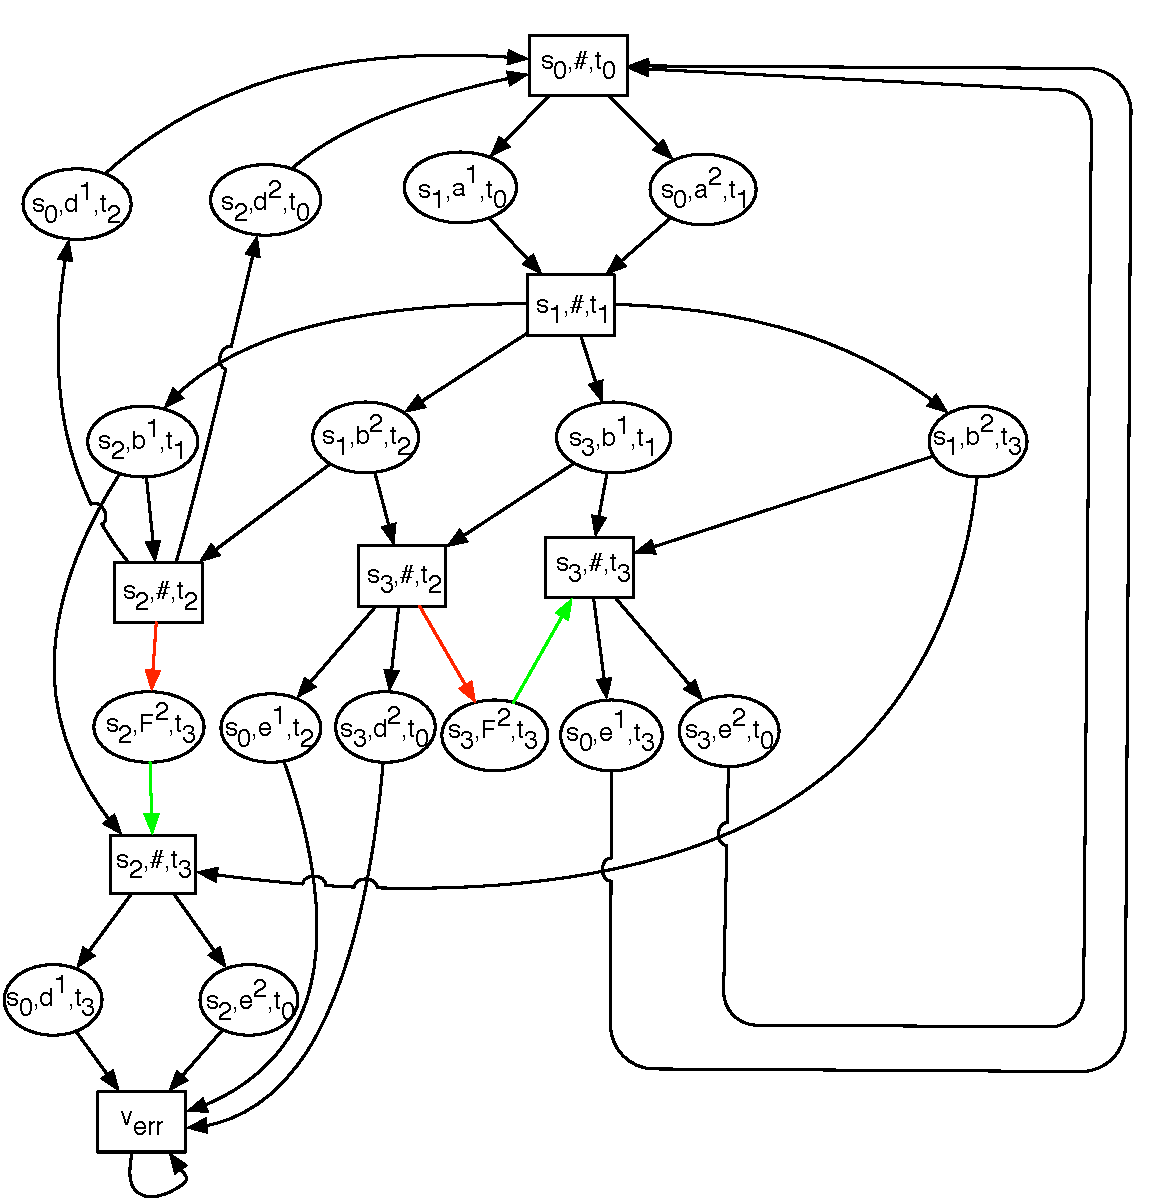
\includegraphics[scale=0.5]{Figs/nondeterm-game-eps-converted-to.pdf} 
%    \caption{Grafo de juego para M y M'}
%    \label{figure:nondeterm-game}
%%\end{figure}

\begin{figure} [ht]
\begin{center}
  %% %\vspace{-0.5cm}
  %% % \includegraphics[scale=0.5]{ex1_cell_mem_game_graph_two_faults.eps} 
  %% \includegraphics[scale=0.5]{ex1_cell_mem_game_graph_two_faults.eps}
  %% %  \vspace{-0.7cm}

  \scalebox{0.8}{
  \begin{tikzpicture}[on grid,auto,align at top,
      hv path/.style={to path={-| (\tikztotarget)},rounded corners},
      vh path/.style={to path={|- (\tikztotarget)},rounded corners},
      hvh path/.style={to path={-- ++(#1,0) |- (\tikztotarget)},rounded corners},
      vhv path/.style={to path={-- ++(0.4,0) |- (\tikztotarget)},rounded corners},
      4giros path/.style={to path={-- ++(0,-1) -- ++(3.5,0) -- ++(0,10.8) -|(\tikztotarget)},rounded corners},
      3giros path/.style={to path={-- ++(0,-0.5) |- ++(1,0) |- (\tikztotarget)},rounded corners}]
    
    \node[rvert] (s0xxxt0)                        {\makebox[4em][c]{$s_0,\#,t_0$}};

    \node[vvert] (s1a1t0) [below=1.7 of s0xxxt0] {\makebox[4em][c]{$s_1,a^1,t_0$}};
    \node[vvert] (s0a2t1) [right=2.0 of s1a1t0]  {\makebox[4em][c]{$s_0,a^2,t_1$}};
    \node[vvert] (s2d2t0) [left=2.0 of s1a1t0]  {\makebox[4em][c]{$s_2,d^2,t_0$}};
    \node[vvert] (s0d1t2) [left=2.0 of s2d2t0]  {\makebox[4em][c]{$s_0,d^1,t_2$}};

    \node[rvert] (s1xxxt1) [below=1.7 of s1a1t0]  {\makebox[4em][c]{$s_1,\#,t_1$}};

    \node[vvert] (s3b1t1) [below=1.7 of s1xxxt1]  {\makebox[4em][c]{$s_3,b^1,t_1$}};
    \node[vvert] (s1b2t3) [right=2.0 of s3b1t1]  {\makebox[4em][c]{$s_1,b^2,t_3$}};
    \node[vvert] (s1b2t2) [left=2.0 of s3b1t1]  {\makebox[4em][c]{$s_1,b^2,t_2$}};
    \node[vvert] (s2b1t1) [left=2.0 of s1b2t2]  {\makebox[4em][c]{$s_2,b^1,t_1$}};

    \node[rvert] (s3xxxt3) [below=1.7 of s1b2t3]  {\makebox[4em][c]{$s_3,\#,t_3$}};
    \node[rvert] (s3xxxt2) [left=2.0 of s3xxxt3]  {\makebox[4em][c]{$s_3,\#,t_2$}};
    \node[rvert] (s2xxxt2) [left=2.0 of s3xxxt2]  {\makebox[4em][c]{$s_2,\#,t_2$}};

    \node[vvert] (s3f2t3) [below=1.7 of s3xxxt3]  {\makebox[4em][c]{$s_3,F^2,t_3$}};
    \node[vvert] (s3d2t0) [left=2.0 of s3f2t3]  {\makebox[4em][c]{$s_3,d^2,t_0$}}; 
    \node[vvert] (s0e1t2) [left=2.0 of s3d2t0]  {\makebox[4em][c]{$s_0,e^1,t_2$}};
    \node[vvert] (s2f2t3) [left=2.0 of s0e1t2]  {\makebox[4em][c]{$s_2,F^2,t_3$}}; 
    \node[vvert] (s0e1t3) [right=2.0 of s3f2t3]  {\makebox[4em][c]{$s_0,e^1,t_3$}};
    \node[vvert] (s3e2t0) [right=2.0 of s0e1t3]  {\makebox[4em][c]{$s_3,e^2,t_0$}};

    \node[rvert] (s2xxxt3) [below=1.7 of s2f2t3]  {\makebox[4em][c]{$s_2,\#,t_3$}};

    \node[vvert] (s0d1t3) [below=1.7 of s2xxxt3]  {\makebox[4em][c]{$s_0,d^1,t_3$}};
    \node[vvert] (s2e2t0) [right=2.0 of s0d1t3]  {\makebox[4em][c]{$s_2,e^2,t_0$}};

    
    
    \node[rvert] (verr)    [below=1.7 of s2e2t0]  {\makebox[4em][c]{$\ErrorSt$}};

    \path[-Latex]
    (s0xxxt0) edge[] (s1a1t0)
    (s0xxxt0) edge[]  (s0a2t1)
    (s2d2t0) edge[]  (s0xxxt0)
    (s0d1t2) edge[]  (s0xxxt0)

    (s1a1t0) edge[]  (s1xxxt1)
    (s0a2t1) edge[]  (s1xxxt1)

    (s1xxxt1) edge[]  (s2b1t1)
    (s1xxxt1) edge[]  (s1b2t2)
    (s1xxxt1) edge[]  (s3b1t1)
    (s1xxxt1) edge[]  (s1b2t3)

    (s2b1t1) edge[bend right=35]  (s2xxxt3)
    (s2b1t1) edge[]  (s2xxxt2)
    (s1b2t2) edge[]  (s2xxxt2)
    (s1b2t2) edge[]  (s3xxxt2)
    (s3b1t1) edge[]  (s3xxxt2)
    (s3b1t1) edge[]  (s3xxxt3)
    (s1b2t3.east) edge[vhv path=-3mm]  (s2xxxt3)
    (s1b2t3) edge[]  (s3xxxt3)
    
    (s2xxxt2) edge[bend left=10]              (s0d1t2)
    (s2xxxt2) edge[bend right=35]              (s2d2t0)
    (s2xxxt2) edge[red]              (s2f2t3)
    (s3xxxt2) edge[]              (s0e1t2)
    (s3xxxt2) edge[]              (s3d2t0)
    (s3xxxt2) edge[red]              (s3f2t3)
    (s3xxxt3) edge[]              (s0e1t3)
    (s3xxxt3) edge[]              (s3e2t0)

    (s2f2t3) edge[darkgreen]              (s2xxxt3)
    (s0e1t2) edge[bend left=36]              (verr)
    (s3d2t0) edge[bend left=32]              (verr)
    (s3f2t3) edge[darkgreen]              (s3xxxt3)
    (s0e1t3.south) edge[4giros path=-3mm]              (s0xxxt0.north)
    (s3e2t0.south) edge[3giros path=-3mm]              (s0xxxt0)

    (s2xxxt3) edge[]              (s0d1t3)
    (s2xxxt3) edge[]              (s2e2t0)
    (s0d1t3) edge[]              (verr)
    (s2e2t0) edge[]              (verr)
    (verr) edge[loop,out=195,in=165,looseness=7]              (verr)
    ;

  \end{tikzpicture}
  }
    
  \caption{Grafo de juego para M y M'.}
  \label{figure:nondeterm-game}
  %\vspace{-0.6cm}
\end{center}
\end{figure}

En este ejemplo, el no-determinismo está dado por la acción $b$. También observemos que hay una falla en $M'$ que conecta los estados $t_2$ y $t_3$. El juego cuantitativo para estos sistemas se muestra en la Figura~\ref{figure:nondeterm-game}. Notemos que cualquier camino más corto en este grafo con respecto a la función de peso $w$ tiene valor $1$ (cualquier camino en el grafo que evite las fallas). Sin embargo, el valor del juego es $\frac{1}{2}$ ya que la mejor estrategia del Refutador es llevar al Verificador al estado $(s_2,b^1,t_1,\Verifier)$. 
Desde ahí, como el Verificador quiere minimizar el valor del juego, su mejor jugada es hacer un movimiento hacia el estado $(s_2,\#,t_2,\Refuter)$. Entonces, el Refutador puede elegir una falla que lleva al estado de error. \\
%Note that the value of this game is $\frac{1}{2}$.\\

La observación anterior sugiere que se necesita un algoritmo diferente para computar la distancia de enmascaramiento para sistemas no deterministas. 
La idea principal es computar los conjuntos $\setsUs$ que fueron definidos en Definición~\ref{def:U} a través de un algoritmo de punto fijo. Para ser más precisos, los conjuntos $\setsUs$ pueden ser calculados utilizando una búsqueda \textit{bottom-up breadth-first} (primero a lo ancho de abajo hacia arriba) desde el estado de error. 
El algoritmo \ref{Alg:MainAlg} muestra el pseudo-código para resolver cualquier juego cuantitativo de enmascaramiento fuerte (resp. débil). 
El algoritmo toma como entrada un grafo de juego cuantitativo de enmascaramiento fuerte  $\QMStrGame = \langle V^G, V_\Refuter, V_\Verifier,E^G, \InitVertex^G, \reward^G \rangle$ 
y computa el valor del juego, es decir, $\val(\QMStrGame)$.
%Let us describe the essential steps of the algorithm for solving any quantitative strong (resp. weak) masking game. 
El algoritmo etiqueta los nodos del grafo con los índices $i$ y $j$. 
%The algorithm can be understood as follows. 
Los pasos principales del algoritmo se detallan a continuación:


\begin{enumerate}
  \item Cada vértice $v$ está etiquetado con un par $(i, j)$ que representa que $v \in U_{i}^{j}$. Inicialmente, $\ErrorSt$ está etiquetado con $(1, 1)$ y todos los demás nodos están etiquetados con $(\infty, \infty)$ (lineas \ref{Alg:InitB}-\ref{Alg:InitE}). 
  Además, utilizamos la asignación $\Q \gets \emptyset$ para denotar la creación de una cola vacía. 
  Después, encolamos el estado de error (lineas \ref{Alg:CreateQ}-\ref{Alg:LoopB}). También mantenemos un conjunto $\STB$ que contiene los estados estabilizados, es decir estados cuyas etiquetas son finales. Los estados que no son alcanzables (hacia atrás) desde el estado de error son ignorados.
  \item Desde el estado de error se lleva a cabo una búsqueda a lo ancho de abajo hacia arriba utilizando una cola de prioridad $\Q$ (lineas \ref{Alg:LoopB}-\ref{Alg:LoopE}), donde el estado con la etiqueta más pequeña (considerando el orden lexicográfico) tiene mayor prioridad. 
  Sea $v'$ el vértice con la prioridad más alta en la cola. Entonces, para todo predecesor $v$ de $v'$ se ejecutan los siguientes pasos (lineas \ref{Alg:LoopBPre}-\ref{Alg:LoopEPre}):
  \begin{itemize}
    \item Si $v$ es un nodo del Verificador (resp. un nodo del Refutador), entonces obtenemos la máxima (resp. mínima) etiqueta $(i,j)$ de todos sus sucesores con respecto al orden lexicográfico. Adicionalmente, si $v$ es un vértice del Verificador y todos sus sucesores están en $\STB$, entonces $v$ se añade al conjunto. En el caso que $v$ sea un vértice del Refutador, 
    el vértice simplemente se añade sin restricción alguna. 
    \item Actualizar el valor de $(i,j)$ incrementando $j$, e incrementando $i$ solo si $\pr{1}{v} \in \Faults$. Llamemos $(i',j')$ a esta nueva etiqueta.
    \item Si $i'$ es diferente del primer componente de la etiqueta actual de $v$, entonces se actualiza y se agrega $v$ a la cola. 
    Observemos que el mismo nodo puede ser añadido a la cola más de una vez a medida que las etiquetas de sus sucesores cambian.
  \end{itemize}
  \item Cuando la cola está vacía, 
  el algoritmo termina y retorna el valor del juego (lineas \ref{Alg:EndB}-\ref{Alg:EndE}). 
  Intuitivamente, el procedimiento termina tan pronto como las etiquetas de todos los estados en el grafo de juego alcanzan su valor final (es decir se alcanza un punto fijo). 
  Sea $k$ la primer componente de la etiqueta del estado inicial, entonces el valor del juego es $\frac{1}{k}$ si 
  $\InitVertex^G \in \STB$, y $0$ en caso contrario.\\
\end{enumerate}
\begin{algorithm}[t!]
\SetAlgoLined
\KwIn{Juego de Enmascaramiento Cuantitativo Fuerte $\QMStrGame = \langle V^G, V_\Refuter, V_\Verifier,E^G, \InitVertex^G, \reward^G \rangle$}
\KwOut{$\val(\QMStrGame)$}
 Etiquetar $\ErrorSt$ con $(1,1)$\; \label{Alg:InitB}
 Etiquetar cada nodo en $V^G \setminus \{\ErrorSt\}$ con $(\infty,\infty)$\; \label{Alg:InitE}
 %$\Q \gets \emptyset$ \tcp*{$\Q$ is a priority queue}  \label{Alg:CreateQ}
 $\Q \gets \emptyset$ \tcp*{$\Q$ es una cola de prioridad}  \label{Alg:CreateQ}
 $\STB \gets \{\ErrorSt\}$\; \label{Alg:CreateSTB}
 %$\mathcal{VE} \longleftarrow \emptyset$\; \label{Alg:CreateVE} 

 $\enqueue(\Q, \ErrorSt)$\; \label{Alg:LoopB} 
 \While{$\Q$ no está vacía}{ \label{Alg:While} 
 	 $v' \gets \dequeue(\Q)$\; \label{Alg:Dequeue-Node}
 	 %\lIf{$\{s'\xrightarrow{\sigma}t \mid t \in post(s')\} \subseteq \mathcal{VE}$}{ \label{Alg:UpdateSTB}
	%	$\mathcal{STB} \longleftarrow \mathcal{STB} \cup \{s'\}$
	 %}
	 
	 \For{$v \in \pre(v') \wedge v \notin \STB$ }{ \label{Alg:LoopBPre}
	 %\For{$s\xrightarrow{\sigma}s' \in E^G$}{ \label{Alg:LoopBPre}
	 	\If{$v \in V_\Verifier$}{
	 		$\lbl \gets \maxlabel(\post(v))$\; \label{Alg:V-Update}
	 		\lIf{$\post(v) \subseteq \STB$}{ \label{Alg:UpdateSTB}
	 		$\STB \gets \STB \cup \{v\}$ 
	 		}
	 		%$enq \longleftarrow post(s) \subseteq \mathcal{STB}$
	 	}
	 	\Else{
	 		$\lbl \gets \minlabel(\post(v))$\; \label{Alg:R-Update}
	 		%$enq \longleftarrow post(s) \cap \mathcal{STB} \neq \emptyset$
	 		$\STB \gets \STB \cup \{v\}$ \label{Alg:R-STB-Update}
	 	}
	 	$\pr{1}{\lbl} \gets \pr{1}{\lbl} + 1$ \tcp*{asumimos $\infty+1=\infty$} \label{Alg:Inc_j}
	 	\lIf{$\pr{1}{v} \in \Faults$}{
	 		$\pr{0}{\lbl} \gets \pr{0}{\lbl} + 1$  \label{Alg:Inc_i}
	 	}
	 	\If{$\pr{0}{\Label(v)} \neq \pr{0}{\lbl}$}{ \label{Alg:Insert-Cond}
	 		Etiquetar $v$ con $\text{lbl}$\;
	 		$\text{Enqueue}(\Q, v)$  \tcp*{$v$ tiene prioridad $\Label(v)$} \label{Alg:Enqueue-Vertex}
	 		%$\mathcal{VE} \longleftarrow \mathcal{VE} \cup \{s\xrightarrow{\sigma}s'\}$
	 	}
	 } \label{Alg:LoopEPre}
 } \label{Alg:LoopE}
 %\lIf{$\pr{0}{Label(s_{0}^G)} \neq \infty$}{ \label{Alg:EndB}
 \lIf{$\InitVertex^G \in \STB$}{ \label{Alg:EndB}
	$\result \gets \frac{1}{\pr{0}{\Label(\InitVertex^G)}}$
 }
 \lElse{
	$\result \gets 0$ \label{Alg:Ret0}
 }
 \Return{$\result$}\; \label{Alg:EndE}
 \caption{Computando el valor del juego de enmascaramiento cuantitativo fuerte} \label{Alg:MainAlg} 
\end{algorithm}


	 Vamos a demostrar que el algoritmo termina y que es correcto.

\sloppy \begin{theorem}\label{thm:alg-termination}  \textbf{(Terminación)} El Algoritmo \ref{Alg:MainAlg} termina.
\end{theorem}
\begin{proof}
Probemos que un vértice no puede ser añadido una cantidad no acotada de veces a $\Q$. 
Primero, observemos que las lineas \ref{Alg:LoopBPre} y \ref{Alg:R-STB-Update} del Algoritmo  \ref{Alg:MainAlg} implican que los vértices del Refutador solo se agregan una vez a la cola. 
Por lo tanto, solo los vértices del Verificador pueden ser añadidos a a $\Q$ una cantidad no acotada de veces.
Probaremos por contradicción que este no es el caso. 
Asumamos que $v$ es un vértice del Verificador que es agregado infinitas veces a la cola. 
Esto implica que $v \notin \STB$ es siempre verdadero dentro del ciclo, y entonces 
$\post(v) \cap (V^G \setminus \STB) \neq \emptyset$ (d lo contrario $v$ seria insertado en $\STB$, linea \ref{Alg:UpdateSTB}). 
Esto significa que,  algún nodo $w \in \post(v)$ del Refutador debe satisfacer $\post(w) \cap \STB = \emptyset$. 
Mas aun, también tenemos $\Label(w) = (\infty, \infty)$ ya que este es el valor inicial que se asigna a $w$, 
y la única manera de modificarlo es ejecutando la linea \ref{Alg:R-Update}, 
en tal caso, $w$ sera agregado a $\Q$, lo cual contradice lo que asumimos. 
Pero la etiqueta de $v$ se calcula siempre tomando el máximo de sus sucesores (linea \ref{Alg:V-Update}), es decir, 
$\Label(v) = (\infty, \infty)$ debe valer dentro del ciclo, y como definimos $\infty + 1 = \infty$, la condición en la linea \ref{Alg:Insert-Cond} siempre es falsa.
Por lo tanto $v$ nunca es agregado a la cola, lo cual contradice nuestro supuesto inicial. 
En resumen, ningún nodo se puede agregar un número no acotado de veces a la cola. Por esto, 
la cola eventualmente se vacía y el algoritmo termina.
\qedhere
\end{proof} 
\sloppy \begin{theorem}\label{thm:alg-correctness} \textbf{(Correctitud)} Al terminar, el Algoritmo \ref{Alg:MainAlg} 
retorna el valor del grafo juego cuantitativo de enmascaramiento fuerte (resp. débil) $\QMStrGame$.
\end{theorem}
% PRUEBA PASADA AL APENDICE
\iffalse
\begin{proof}
Consideremos la función  $\delta(v) = \min \{(i,j) \mid v \in \setsUs\}$, donde $\min \emptyset = (\infty, \infty)$.
También consideramos la extensión de esta función a conjuntos, es decir, $\delta(W) = \{\delta(w) \mid w \in W \}$. 
Además, las siguientes propiedades de $\delta$ son una consecuencia de la definición \ref{def:U}: \\

\noindent
Si $v$ es un vértice del Refutador:
\begin{equation}\label{prop:delta-1}
 \delta(v)  = \min \{(i,j+1) \mid (i,j) \in \delta(\post(v)) \}
\end{equation}
Si $v$ es un vértice del Verificador y $\pr{1}{v} \in \Faults$ entonces:
\begin{equation}\label{prop:delta-2}
 \delta(v)  = \max \{(i+1,j+1) \mid (i,j) \in \delta(\post(v)) \}
\end{equation}
Si $v$ es un vértice del Verificador y $\pr{1}{v} \notin \Faults$ entonces:
\begin{equation}\label{prop:delta-3}
 \delta(v) = \max \{(i,j+1) \mid (i,j) \in \delta(\post(v)) \}
\end{equation}
	Ahora bien, probemos que los siguientes predicados siempre valen después de la linea \ref{Alg:While}.
\begin{equation}\label{Alg:inv0}
	\forall v \in \STB : \Label(v) < (\infty, \infty)
\end{equation}
\begin{equation}\label{Alg:inv1}
	\forall w, v \in S^G : v \in \STB \wedge \Label(w) < \Label(v) \Rightarrow w \in \STB
\end{equation}
%and 
\begin{equation}\label{Alg:inv2}
	\forall v \in \STB : \Label(v) = \delta(v)
\end{equation}

Prueba de la propiedad \ref{Alg:inv0}: vale para la inicialización (linea \ref{Alg:CreateSTB}). Vamos a hacer la prueba por contradicción. 
Sea $v$ el primer nodo agregado a $\STB$ tal que $\Label(v) = (\infty, \infty)$.
Si es un vértice del Refutador, entonces $\post(v) \cap \STB \neq \emptyset$ y como $v$ era el primer nodo agregado a $\STB$ con 
$\Label(v) = (\infty, \infty)$ tenemos que $\forall w \in \post(v) \cap \STB: \Label(w) < (\infty, \infty)$. Pero entonces, en la linea \ref{Alg:R-Update},
$v$ es etiquetado con una etiqueta diferente de $(\infty, \infty)$ lo cual es una contradicción. 
De forma similar, si $v$ es un vértice del Verificador, entonces $\post(v) \subseteq \STB$ y 
por lo tanto se lo etiqueta en la linea \ref{Alg:V-Update} con un valor diferente de $(\infty, \infty)$, lo cual contradice nuestro supuesto inicial. 
Por consiguiente, $\forall v \in \STB : \Label(v) < (\infty, \infty)$.

Prueba de la propiedad \ref{Alg:inv1}: $\STB$ se inicializa con $\{\ErrorSt \}$ y por lo tanto la propiedad vale antes de la linea \ref{Alg:While}. 
De nuevo hacemos la prueba por contradicción, asumamos que $v$ es el primer nodo agregado a $\STB$ que no cumple con la propiedad, es decir, existe un $w$ tal que $\Label(w) < \Label(v)$ y
$w \notin \STB$; además, asumamos que $w$ es e vértice con la etiqueta mas pequeña que satisface esto. 
Como $v \in \STB$ tenemos $\Label(v)<(\infty, \infty)$ (por Prop.~\ref{Alg:inv0}) y entonces $\Label(w)< (\infty, \infty)$. 
De hecho, $w$ no puede ser un vértice del Refutador, de lo contrario, al ser etiquetado, tendría que ser agregado a $\STB$ (linea \ref{Alg:R-STB-Update}), 
contradiciendo nuestros supuestos. 
Ahora bien, si $w$ es un vértice del Verificado y $\Label(w) < (\infty, \infty)$
ya que $\Label(w) = \max\{\Label(z) \mid z \in \post(w)\}$ (linea \ref{Alg:R-Update}), tenemos: $\forall z \in \post(w) : \Label(z) < (\infty, \infty)$.
Además, por transitividad tenemos que $\forall z \in \post(w) : \Label(z) < \Label(v)$. Pero como asumimos que 
$w$ era el vértice con la menor etiqueta que satisface $\Label(w) < \Label(v)$ y $w \notin \STB$, tenemos que $\forall z \in \post(v) : z \in \STB$. Pero entonces cuando $v$ fue inspeccionado en la linea \ref{Alg:UpdateSTB} este fue agregado a $\STB$, 
lo cual lleva a una contradicción.

Prueba de la Propiedad \ref{Alg:inv2}: la propiedad vale para $\ErrorSt$. Sea $v$ el primer vértice agregado a $\STB$ tal que $\Label(v) \neq \delta(v)$. En el caso que $v$ es un vértice del Verificador, entonces, como $v \in \STB$, tenemos $\post(v) \subseteq \STB$. Además, asumimos que $v$ era el primer vértice que viola esta propiedad, entonces tenemos que $\forall w \in \post(v):\delta(w)=\Label(w)$. Además, si $\pr{1}{v} \notin \Faults$, entonces: 
\begin{align*}
\Label(v) & = \max \{(i,j+1) \mid (i,j) \in \Label(\post(v))\}&  \text{(Lineas \ref{Alg:V-Update} y \ref{Alg:Inc_j})}\\
	      & =  \max \{(i,j+1) \mid (i,j) \in \delta(\post(v))\}&  \text{(Suposición)}\\
	      & = \delta(v)& \text{(Prop. \ref{prop:delta-3})}
\end{align*}
lo cual es una contradicción. Ahora bien, en el caso que $\pr{1}{v} \in \Faults$ tenemos que:
\begin{align*}
\Label(v) & = \max \{(i+1,j+1) \mid (i,j) \in \Label(\post(v))\}&  \text{(Lineas \ref{Alg:V-Update}, \ref{Alg:Inc_j}, y \ref{Alg:Inc_i})}\\
	      & =  \max \{(i+1,j+1) \mid (i,j) \in \delta(\post(v))\}&  \text{(Suposición)}\\
	      & = \delta(v)& \text{(Prop. \ref{prop:delta-2})}
\end{align*}
lo cual también contradice nuestra suposición. Por lo tanto, $v$ no puede ser un vértice del Verificador. 
En el caso que $v$ sea un vértice del Refutador, como $v \in \STB$ tenemos que $\Label(v) < (\infty, \infty)$ por la Prop.~\ref{Alg:inv0}. 
Por lo tanto, cuando $v$ fue agregado a $\STB$, $\Label(v) = \min\{ \Label(w) \mid w \in \post(v)\}$. Por consiguiente, 
existe un $w \in \post(v)$ tal que $\Label(w) \leq \Label(v)$, pero entonces por la Prop.~\ref{Alg:inv1} 
tenemos $w \in \STB$. De este modo:
\begin{align*}
\Label(v) & = \min \{(i,j+1) \mid (i,j) \in \Label(\post(v))\}&  \text{(Lineas \ref{Alg:R-Update} y \ref{Alg:Inc_j})} \\
	      & =  \min \{(i,j+1) \mid (i,j) \in \delta(\post(v))\}&  \text{(Suposición)}\\
	      & = \delta(v)& \text{(Prop. \ref{prop:delta-2})}
\end{align*}
lo cual contradice nuestras suposiciones. Por esto, $\Label(v) = \delta(v)$.

Ahora bien, vamos a probar que cuando el ciclo de la linea \ref{Alg:LoopBPre} termina tenemos:
\begin{equation}\label{Alg:inv3}
 \forall v \in S^G \setminus \STB : \delta(v)=(\infty, \infty)
\end{equation}

Vamos a hacer la prueba por contradicción. Sea $v \in S^G \setminus \STB$ tal que $\delta(v) < (\infty, \infty)$ y, además, asumamos que
%$\delta(v) = \min \{w \in S^G \setminus \STB \mid \delta(w) < (\infty, \infty) \}$.
$\delta(v)$ es la etiqueta mas pequeña que satisface esto.
Si $v$ es un vértice del Refutador, entonces existe algún $w \in \post(v)$ tal que $\delta(w) < \delta(v)$. 
Por lo tanto, tenemos que $w \in \STB$ (por nuestra suposición) lo cual significa que $v$ fue agregado al menos una vez a la cola ya que fue inicializado con $(\infty, \infty)$. 
De este modo, fue agregado a $\STB$ en la linea \ref{Alg:R-STB-Update}, lo cual contradice nuestro supuesto inicial. 
Por lo tanto, $v$ debe ser un vértice del Verificador. 
Si $\pr{1}{v} \in \Faults$, entonces $\delta(v) = \max \{(i+1,j+1) \mid (i,j) \in \delta(\post(v))\}$ 
y por lo tanto $\delta(v) > \delta(w)$ para todo $w \in \post(w)$.
Entonces, por nuestras suposiciones, $w \in \STB$ para todo $w \in \post(v)$.
Además, cuando el ultimo $w \in \post(v)$ fue agregado a $\STB$, $v$ estuvo en la cola debido a la política de recorrido primero en lo ancho (BFS).
De hecho, cuando la condición $\post(v) \subseteq \STB$ fue evaluada para $v$ (linea \ref{Alg:UpdateSTB}), es verdadera y entonces $v$ 
debería ser agregado a $\STB$, contradiciendo nuestra suposición. Por lo tanto, $v \in \STB$.

Finalmente, el resultado computado por el Algoritmo \ref{Alg:MainAlg} se deduce de las propiedades \ref{Alg:inv2}, \ref{Alg:inv3}, 
y el Teorema \ref{thm:quant_game}. 
Entrando mas en detalle, si $\delta(s_{0}^G) = (\infty, \infty)$, entonces por Prop. ~\ref{Alg:inv0} y \ref{Alg:inv3}, tenemos que cuando termina, $\Label(s_{0}^G) = (\infty, \infty)$. 
De este modo, el algoritmo retorna $0$ en la linea \ref{Alg:Ret0} lo cual es correcto por el Teorema~\ref{thm:quant_game}. 
En el caso que $\delta(s_0^G)< (\infty, \infty)$, entonces $s_0^G \in \STB$ y también que Prop.~\ref{Alg:inv2} tenemos $\Label(v) = \delta(v)$. Por lo tanto, el algoritmo retorna el resultado correcto en la linea \ref{Alg:EndB} por el Teorema \ref{thm:quant_game}. 
\qedhere
\end{proof}
\fi




Nos queda discutir la complejidad del tiempo de ejecución para computar el valor de juegos cuantitativos de enmascaramiento. 
El siguiente teorema establece cual es la complejidad de determinar el valor de cualquier tipo de juegos cuantitativos de enmascaramiento.
%
%\noindent
%Finally, winning regions (and strategies) can be computed in lineal time.  
\sloppy \begin{theorem}\label{thm:qgame-determined} Cualquier grafo de juego cuantitativo de enmascaramiento fuerte (resp. débil) 
$\QMStrGame = \langle V^G, V_\Refuter, V_\Verifier, E^G, \InitVertex^G, \reward^G \rangle$ puede ser determinado en tiempo $\BigO(|E^G|*\log |V^G|)$ (resp. $\BigO(|E_W^G|*\log |V^G|)$).
\end{theorem}
\begin{proof}
Notemos que el ciclo de la linea \ref{Alg:LoopBPre} inspecciona los arcos del grafo. Además, notemos que, ningún arco $(v, v')$ se puede inspeccionar dos veces:
si $v'$ es un vértice del Refutador, entonces sera agregado a $\STB$ y el arco no puede ser procesado nuevamente. 
Si $v$ es un vértice del Verificador, entonces $v'$ es un vértice del Refutador, por lo que una vez desencolado (linea \ref{Alg:Dequeue-Node}), no será agregado a la cola de nuevo, y por lo tanto el arco $(v, v')$ no sera procesado de nuevo. Por esto, el ciclo de la linea \ref{Alg:LoopBPre} será ejecutado $|E^G|$ veces en el peor caso. 
Además, si se utiliza una implementación eficiente de colas de prioridad para almacenar los estados (linea \ref{Alg:Enqueue-Vertex}), entonces tomaría $\BigO(\log |V^G|)$ pasos la inserción o eliminación de un elemento en la cola, es decir, en total, el ciclo de la linea \ref{Alg:LoopBPre} toma $\BigO(|E^G|*\log |V^G|)$ pasos.
Adicionalmente, notemos que el \emph{ciclo while} de la linea \ref{Alg:While} se ejecuta hasta que $\Q$ se vacíe, y los nodos solo son encolados en la linea \ref{Alg:Enqueue-Vertex}. Por lo tanto, la cantidad de veces que el \emph{ciclo while} es ejecutado está acotado por el numero de veces que el \emph{ciclo for} es ejecutado, lo cual implica que el ciclo exterior es ejecutado a lo sumo $O(|E^G|)$ veces. Estas consideraciones son similares para el caso de los juegos cuantitativos de enmascaramiento débil.	

\qedhere
\end{proof} \\
% TBD similar for weak games

Los Teoremas \ref{thm:game-determined} y \ref{thm:qgame-determined} describen la complejidad de resolver los juegos de enmascaramiento estándar y cuantitativos respectivamente. Sin embargo, en la práctica, uno necesita tener en cuenta que $|V^G| = |S|*|S'|$ y $|E^G| = |{\rightarrow}|+|{\rightarrow'}|$, así que construir el juego toma 
$\BigO(|S|^2*|S'|^2)$ pasos en el peor caso. Adicionalmente, para juegos débiles, la clausura transitiva del modelo original necesita ser computada, lo cual cuesta $\BigO(\max(|S|,|S'|)^{2.3727})$ para el mejor algoritmo conocido \cite{Wil12}.

Es interesante destacar que los juegos deterministas pueden ser resueltos en tiempo lineal utilizando el hecho demostrado en el Teorema \ref{thm:det-games}.
\begin{theorem}\label{thm:deterministic-qgame-complexity} 
Cualquier juego de enmascaramiento determinista fuerte (resp. débil) puede ser resuelto en tiempo $\BigO(|E^G|)$ (resp. $\BigO(|E_W^G|)$).
\end{theorem}
\begin{proof} Por el Teorema \ref{thm:det-games}, el valor del juego está dado por el camino mas corto hacia el estado de error en el grafo de juego donde la función de peso asigna $1$ a las fallas, y $0$ a otras transiciones. El algoritmo de Dial \cite{Dial69} puede ser utilizado para obtener el camino mas corto en este grafo, el cual tiene complejidad $\BigO(|E^G|)$  (resp. $\BigO(|E^G_W|)$ en el caso de los juegos débiles).
\qedhere
\end{proof} 

Observemos que al utilizar los conjuntos $\setsUs$ podemos definir estrategias óptimas para el Refutador y el Verificador, sin tener en cuenta la historia de la jugada. Esto significa que podemos dar el siguiente teorema.
 
\begin{theorem} \label{thm:memoryless} Sea $\QMStrGame$ un grafo de juego cuantitativo de enmascaramiento fuerte.
  Los jugadores $\Refuter$ y $\Verifier$ tienen estrategias óptimas sin memoria para $\QMStrGame$.
\end{theorem}
\begin{proof} Para un juego dado podemos computar los conjuntos $\setsUs$ utilizando el Algoritmo~\ref{Alg:MainAlg}.
Por esto, se puede definir de forma directa una estrategia óptima para el Refutador. 
Para un nodo dado $v$, si este pertenece a algún $\setsUs$, entonces el Refutador elige algún nodo en $U^{j'}_{i'}$ donde: 
$(i', j') = \text{max}\{(i'', j'') \mid post(v) \cap U^{j}_{i} \neq \emptyset \wedge (i'',j'') < (i,j) \}$. 
Por definición de $\setsUs$, sabemos que el susodicho par existe, y también que esta estrategia es ganadora para el Refutador. Si $v \notin \setsUs$, entonces cualquier elección del Refutador llevará a una jugada ganadora del Verificador. 
Por lo tanto, el Refutador se mueve a cualquier sucesor de $v$.
De forma similar, podemos definir una estrategia óptima para el Verificador.
\qedhere 
\end{proof} \\

%% \noindent
%% Now, we present some basic properties of the masking distance.

Al utilizar $\QMWeakGame$ en lugar de $\QMStrGame$ en la 
Definición~\ref{def:mask_dist}, podemos definir la \emph{distancia de enmascaramiento débil} $\DeltaMask^W$. El próximo teorema establece que $A$ y
$A'$ están a distancia $0$ si y solo si existe una simulación de enmascaramiento fuerte (o débil) entre ellos.

\begin{theorem}\label{thm:ref}
  Para cualquier par de sistemas de transición $A = \langle S, \Sigma, \rightarrow, \InitState \rangle$ y $A' = \langle S', \Sigma_{\mathcal{F'}}, \rightarrow', \InitStatePrime \rangle$, vale que:
  \begin{enumerate}[(i)]
  \item  $\DeltaMask(A,A') = 0$ si y solo si $A \Masking A'$, y
   \item $\DeltaMask^W(A,A') = 0$ si y solo si $A \WeakMasking A' $.
  \end{enumerate}
\end{theorem}
%
Esto se deduce del Teorema \ref{thm:quant_game}.
%That is, the masking distance between two systems is $0$ if and only if there is a masking simulation between them.
Si notamos que $A \Masking A$ (y $A \WeakMasking A$) para cualquier sistema de transición $A$, obtenemos que $\DeltaMask(A,A)=0$ (resp.\ $\DeltaMask^W(A,A)=0$) por el Teorema \ref{thm:ref}, es decir, 
las dos distancias son reflexivas.

Para nuestro ejemplo de la celda de memoria, la distancia de enmascaramiento es de $1/3$ 
con una redundancia de $3$ bits y considerando que pueden ocurrir al menos dos fallas. 
Esto significa que solo una falla pudo ser enmascarada de forma exitosa por esta implementación. \\

Podemos probar una versión de la desigualdad triangular para nuestra noción de distancia.
%
\begin{theorem} \label{thm:triang_ineq}
Sean $A = \langle S, \Sigma, \rightarrow, s_0 \rangle$, $A' = \langle S', \Sigma_{\mathcal{F'}}, \rightarrow', s'_0 \rangle$,  y  $A'' = \langle S'', \Sigma_{\mathcal{F''}},\rightarrow'', s''_0 \rangle$ unos sistemas de transición tales que $\Faults' \subseteq \Faults''$, y los juegos correspondientes $\mathcal{Q}_{A,A'}$, $\mathcal{Q}_{A',A''}$ y $\mathcal{Q}_{A,A''}$.
Entonces $\DeltaMask(A,A'') \leq \DeltaMask(A,A') + \DeltaMask(A', A'')$ y $\DeltaMask^W(A,A'') \leq \DeltaMask^W(A,A') + \DeltaMask^W(A', A'').$
\end{theorem}
\iffalse
% PRUEBA PASADA AL APENDICE
\begin{proof} 
Probaremos que para cualquier nodo $(s,\#,s'',\Refuter)$ en $\mathcal{Q}_{A,A''}$ y para cualquier par de nodos
$(s,\#, s', R)$ en $\QMStrGame$ y $(s',\#,s'', R)$ en $\mathcal{Q}_{{A'},A''}$ (para cualquier estado $s'$ en $A'$), se cumple que:
\[
\frac{1}{\pr{0}{\delta((s,\#, s'', \Refuter))}} \leq \frac{1}{\pr{0}{(\delta(s,\#, s', R))}} + \frac{1}{\pr{0}{\delta((s',\#, s'', R))}}
\] 
donde $\delta(v) = \min \{(i,j) \mid v \in U^i_j\}$, calculado en el juego correspondiente. 
Como en el Teorema \ref{thm:quant_game}, solo definimos $\max \emptyset = (\infty, \infty)$. 
El resultado se deduce de este hecho y el Teorema \ref{thm:quant_game}. La prueba es por inducción sobre $\delta((s,\#, s'', \Refuter))$.

Primero, observemos que para cualquier nodo $(s, \#, s'', \Refuter)$ del juego $\mathcal{Q}_{A,A''}$ debemos tener $\delta((s, \#, s'', \Refuter)) \geq (1,3)$.
De hecho, este nodo no puede ser el estado de error, lo cual significa que $j \neq 1$. Además, luego del movimiento del Refutador tenemos al menos un movimiento del Verificador y por lo tanto $j \geq 3$. Es decir que el caso base es $\delta((s,\#, s'', \Refuter)) = (1,3)$.
\begin{description}
\item [Caso Base] Si $\delta((s,\#, s'', \Refuter)) = (1,3)$. Asumamos que $(s, \#, s'', R) \in U^3_1$. Esto significa que tenemos una transición 
$((s, \#, s'', \Refuter), (w, \sigma^t, w'', \Verifier))$, donde $t \in \{1,2\}$, que no puede ser emparejada por el Verificador. 
En el caso que $t=1$, entonces este movimiento es una transición $((s, \#, s'', \Refuter), (w, \sigma^1, s'', \Verifier))$ de $A$. 
Ahora bien, sean $(s, \#, s', \Refuter)$ y $(s', \#, s'', \Refuter)$ un par de estados de $\QMStrGame$ y $\mathcal{Q}_{A',A''}$, respectivamente. 
Por definición, tenemos una transición $((s, \#, s', \Refuter), (w, \sigma^1, s', \Verifier))$ en $Q_{A,A'}$. 
En el caso que el Verificador no pueda emparejar este movimiento en ese juego, tenemos que $(s, \#, s', \Refuter) \in U^3_1$. 
Esto finaliza la prueba ya que $1 \leq 1 + k''$, independientemente del valor de $k''$. 
De lo contrario, el Verificador escoge un movimiento que empareja al de su contrincante, es decir, $((w, \sigma^1, s', \Verifier), (w, \#, w', \Refuter))$ en $\mathcal{Q}_{A,A'}$. 
Además, tenemos una transición $((s', \#, s'', \Refuter), (w', \sigma^1, s'', \Verifier))$ en $\mathcal{Q}_{A',A''}$. 
Pero, esta no puede ser emparejada debido a nuestro supuesto inicial. Por lo tanto, $\delta((s', \#, s'', \Refuter))= (1,3)$, y tenemos que:
\begin{align*}
	\frac{1}{\pr{0}{\delta((s,\#, s'', \Refuter))}}  & = 1\\
							& \leq \frac{1}{\pr{0}{\delta((s, \#, s', \Refuter))}} + 1\\
							& =   \frac{1}{\pr{0}{\delta((s, \#, s', \Refuter))}}  + \frac{1}{\pr{0}{\delta((s', \#, s'', \Refuter))}}
\end{align*}
Para $t=2$,  el razonamiento es similar usando las transiciones de $A''$. 

\item [Paso Inductivo] Para $(i,j) > (1,3)$ la prueba es como sigue. 
Asumamos que $\delta((s, \#, s'', \Refuter)) = (i,j)$. Como $1<i \leq j$, tenemos una transición 
$((s, \#, s'', \Refuter), (w, \sigma^t, w'', \Verifier))$ en $\mathcal{Q}_{A,A''}$. vamos a proceder por casos.

  En el caso $\sigma^t = F^2$ para algún $F \in \Faults''$. Como $\delta((s, \#, s'', \Refuter)) > (1,3)$,
debemos tener una transición $((s, F^2, w'', \Verifier), (s, \#, w'', \Refuter)) \in Q_{A,A''}$ y $\delta((s, \#, w'', \Refuter)) = (i-1,j-2)$. 
Por lo tanto, por definición de $\mathcal{Q}_{A',A''}$, tenemos una transición 
$((s', \#, s'', \Refuter), (s', F^2, w'', \Verifier))$ en $\mathcal{Q}_{A',A''}$. 
En el caso de que $F \in \Faults'$, entonces $F \in \Sigma_{\Faults'}$. 
Si no puede ser emparejada, entonces:
\begin{align*}
\frac{1}{\pr{0}{\delta((s,\#, s'', \Refuter))}}  & \leq 1	\\
							     &= \frac{1}{\pr{0}{\delta((s', \#, s'', \Refuter))}}  \\
							     &\leq  \frac{1}{\pr{0}{\delta((s, \#, s', \Refuter))}} +  \frac{1}{\pr{0}{\delta((s', \#, s'', \Refuter))}}   
\end{align*}
y el resultado se deduce. De lo contrario, tenemos una colección de transiciones  $((s', F^2, w'', \Verifier), (w', \#, w'', \Refuter))$ en $\mathcal{Q}_{A',A''}$. 
Así que, en el juego $\QMStrGame$, tenemos al menos un arco $((s, \#, s', \Refuter), (s, F^2, w', \Verifier))$. 
Entonces, como $((s, F^2, w'', \Verifier), (s, \#, w'', \Refuter)) \in Q_{A,A''}$, también tenemos una transición $((s, F^2, w', \Verifier), (s, \#, w', \Refuter))$ en $Q_{A,A'}$. 
Por hipótesis inductiva, tenemos $\delta((s, \#, w', \Refuter))= i'$ y $\max \{ \delta(v) \mid v \in \post((s', F^2, w'', \Verifier)) \}=i''$ tal que:
\begin{equation}\label{eq:hi1}
\frac{1}{i-1} \leq \frac{1}{i'} + \frac{1}{i''}.
\end{equation} 
y por lo tanto:
\begin{equation}\label{eq:hi1a}
\frac{1}{i} \leq \frac{1}{i'+1} + \frac{1}{i''}.
\end{equation}
Además, notemos que $\delta((s, F^2, w', \Verifier)) \geq (i'+1,j'+1)$ y tenemos una transición (de enmascaramiento) única desde $(s, F^2, w', \Verifier)$. 
De este modo, 
\begin{equation}\label{eq:hi2}
	\delta((s, \#, s', \Refuter)) \geq (i'+1,j'+2)
\end{equation}
De manera similar, como $F \in \Sigma_{\Faults'}$ tenemos que:
\begin{equation}\label{eq:hi3}
	\delta((s', \#, s'', \Refuter)) \geq (i'',j'+2)
\end{equation}
Por esto, teniendo en cuenta las inecuaciones \ref{eq:hi1a}, \ref{eq:hi2} y \ref{eq:hi3}, obtenemos:
\begin{align*}
	\frac{1}{\pr{0}{\delta((s,\#, s'', \Refuter))}} & = \frac{1}{i} & \text{(Suposición)} \\
									      & \leq \frac{1}{i'+1} + \frac{1}{i''} & \text{Ineq.~\ref{eq:hi1a}} \\
									      &  = \frac{1}{\pr{0}{\delta((s, \#, s', \Refuter))}} \ +  \\ &\phantom{=\ } \frac{1}{\pr{0}{\delta((s', \#, s'', \Refuter))}} &
\end{align*}
	Si $F \notin \Faults'$, entonces debemos tener una transición $((s', F^2, w'', \Verifier), (s', \#, w'', \Refuter))$ en $\mathcal{Q}_{A',A''}$. 
Ahora bien, por hipótesis inductiva, tenemos $\delta((s, \#, s', \Refuter)) = (i',j')$ y $\delta((s', \#, w'', \Refuter)) = (i'',j'')$ tal que 
$\frac{1}{i-1} \leq \frac{1}{i'} + \frac{1}{i''}$. De este modo, $\delta((s', \#, s'', \Refuter)) = (i''+1, j''+2)$ y de forma similar a lo previo, el resultado se deduce.

	En el caso $\sigma^t \neq F^2$. Si $t=1$, entonces tenemos una transición $((s, \#, s'', R), (w, \sigma^1, s'', V))$ en $\mathcal{Q}_{A,A''}$, y 
	como $\delta((s, \#, s'', \Refuter)) > (1,3)$,
debemos tener una transición $((s, \sigma^1, w'', \Verifier), (w, \#, w'', \Refuter))$ en $Q_{A,A''}$ tal que $\delta((s, \#, w'', \Refuter)) = (i,j-2)$. 
Por definición del juego $Q_{A, A'}$, tenemos una transición
$((s, \#, s', \Refuter), (w, \sigma^1, s', \Verifier))$. En el caso que no pueda ser emparejada, entonces esta lleva al resultado que buscamos. De lo contrario, vamos a definir $(i',j') = \max \{\delta(v) \mid v \in \post((w, \sigma^1, s', \Verifier)) \}$. 
Como $\post((w, \sigma^1, s', \Verifier)) \neq \{\ErrorSt\}$, también debe existir una transición $((s', \#, s'', R), (w', \sigma^1, s'', V))$ en $Q_{A',A''}$. 
En el caso que esta no pueda ser emparejada, entonces tenemos $\delta((s', \#, s'', R)) = (1,3)$ y la prueba finaliza. 
En otro caso, definamos $i'' = \max \{\delta(v) \mid v \in \post((w', \sigma^1, s'', V)) \}$ donde por hipótesis inductiva tenemos
\begin{equation}
	\frac{1}{i} \leq \frac{1}{i'} + \frac{1}{i''}
\end{equation}	
	Por esto, 
\begin{equation}
	\frac{1}{\pr{0}{\delta((s, \#, s'', R))}} \leq \frac{1}{\pr{0}{\delta((s, \#, s', R))}} + \frac{1}{\pr{0}{\delta((s', \#, s'', R))}}
\end{equation}	
	Para el caso $t=2$ la prueba es similar.
\end{description}


\qedhere
\end{proof}\\
\fi

La prueba para $\DeltaMask^W$ es similar a la de $\DeltaMask$ 
pero utilizando $\QMWeakGame$ en lugar de $\QMStrGame$ y por el Teorema~\ref{thm:weak_thm}.

Las propiedades de reflexividad y desigualdad triangular implican que ambas distancias de enmascaramiento son semi-métricas dirigidas \cite{CharikarMM06,AlfaroMRS08}. Además, es interesante destacar que la propiedad de desigualdad triangular tiene aplicaciones prácticas interesantes. Al momento de desarrollar software crítico es bastante común desarrollar una primera versión del software teniendo en cuenta algunas posibles fallas anticipadas. 
Luego, después de una fase de \textit{testing} y de la ejecución misma del sistema, es posible que más fallas puedan ser observadas. En consecuencia, el sistema es modificado con nuevos mecanismos de tolerancia a fallas para tolerar estas nuevas fallas observadas. 
El Teorema \ref{thm:triang_ineq} establece que ir midiendo la distancia de enmascaramiento de estas diferentes versiones del software de manera incremental provee una cota superior de la distancia entre el sistema nominal y la última versión de su implementación tolerante a fallas. Esto significa que, si la suma de las distancias obtenidas entre diferentes versiones es un número pequeño, entonces podemos asegurar que la versión final del sistema exhibirá una tolerancia a fallas enmascarante aceptable con respecto al sistema nominal.